\documentclass[10pt]{beamer}

\usetheme[progressbar=frametitle]{metropolis}
\usepackage{appendixnumberbeamer}

\usepackage{booktabs}
\usepackage[scale=2]{ccicons}

\usepackage{pgfplots}
\usepgfplotslibrary{dateplot}

\usepackage{xspace}
\newcommand{\themename}{\textbf{\textsc{metropolis}}\xspace}

\title{The Pinksy-Rinzel Model and Parameter Estimation}

\date{\today}

\author{Matthias Heinkenschloss, Arjun Sethi-Olowin}
\institute{Department of Computational and Applied Mathematics and Operations Research\\Rice University, Houston, Texas}
% \titlegraphic{\hfill\includegraphics[height=1.5cm]{logo.pdf}}

\begin{document}

\maketitle

\begin{frame}{Table of contents}
  \setbeamertemplate{section in toc}[sections numbered]
  \tableofcontents%[hideallsubsections]
\end{frame}

\section[Pinsky-Rinzel Model]{Pinsky-Rinzel Model}

\begin{frame}[fragile]{Overview of the Model}

    \begin{itemize}
        \item A system of differential equations
        \item Models behavior of the CA3 neurons in the hippocampus
        \item Split into a somatic compartment and a dendritic compartment
    \end{itemize}
    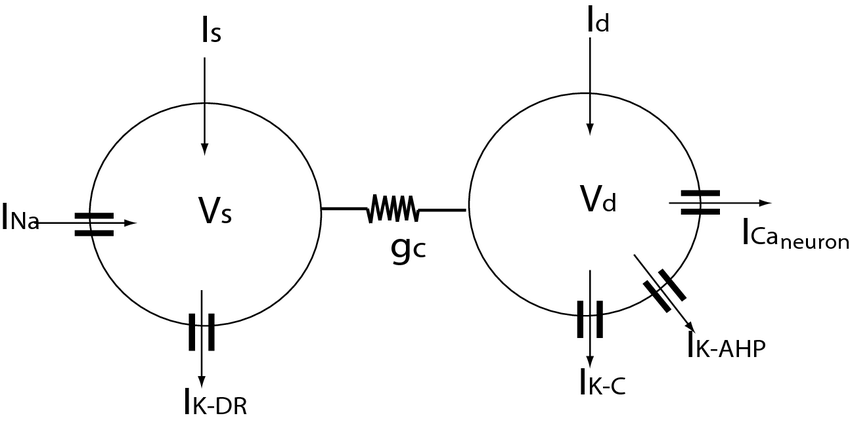
\includegraphics[width=0.7\textwidth]{Latex/Schematic_Pinsky-Rinzel_Model.png}
\end{frame}

\begin{frame}{Two-Compartment Model}
    ADD EQUATIONS (maybe not all?)
\end{frame}

\section{Parameters and constants}

\begin{frame}{Knowns}
	We know constants which are...\\
    have some parameters which are constant in time, but value is undetermined\\
    functions?
\end{frame}

\section{Two-Compartment Code}

\begin{frame}[Simulation]
    Simulation code where we provide parameter values to understand how various functions in the model change
\end{frame}

\begin{frame}[Pyomo]
    Pyomo code solves parameters to minimize error for function values over time compared to collected data
\end{frame}

\section{Conclusion}

\begin{frame}{Summary}
    
\end{frame}

\begin{frame}{Next Steps}
    Pyomo stuff
\end{frame}
    


\appendix

\begin{frame}{References}

    references here
    
\end{frame}

\end{document}
